\chapter{Introducci\'on}
\label{cap:intro}

El presente capítulo se desarrolla el planteamiento del problema, para lo cual es necesario explorar el contexto general; antecedentes, motivaciones y las principales características de la solución propuesta.

Algunos de los elementos más motivadores para el desarrollo de un proyecto como este son sin duda, aquellos relacionados con las potenciales aplicaciones que puede tener un detector de peatones. Algunos de los ejemplos clásicos de estas aplicaciones son aquellos relacionados con la video vigilancia. Sin embargo, existen gran variedad de aplicaciones que hoy se encuentran en auge, por ejemplo las relacionadas con automóviles que se conducen de forma autónoma, o a tareas realizadas por vehículos aéreos no tripulados, por esto es importante la continua búsqueda de mejoras para los algoritmos de detección.

\section{Antecedentes y motivación}
\label{intro:motivacion}

Para un ser humano el proceso de visión resulta un ejercicio bastante simple. Este es capaz de distinguir cuantas personas hay en una imagen sin esforzarse demasiado aún en condiciones desfavorables tales como, una imagen borrosa o con poca luz. La visión humana es un sentido complejo que abarca la habilidad de detección de la luz y su posterior interpretación en imágenes. Esta función es realizada a través del ojo, que capta la energía lumínica, transformándola en señales eléctricas que son recibidas por la corteza cerebral.
La luz se identifica inicialmente mediante determinadas longitudes de onda, distinguiéndose la percepción de los colores mediante el espectro electromagnético. El ojo humano es capaz de captar desde el rojo (700 nm) hasta el violeta (400 nm), ubicándose más allá de estos límites el espectro infrarrojo y ultravioleta, respectivamente (ver figura~\ref{fig:espectro}).

\begin{figure}[htc]
  \centering
  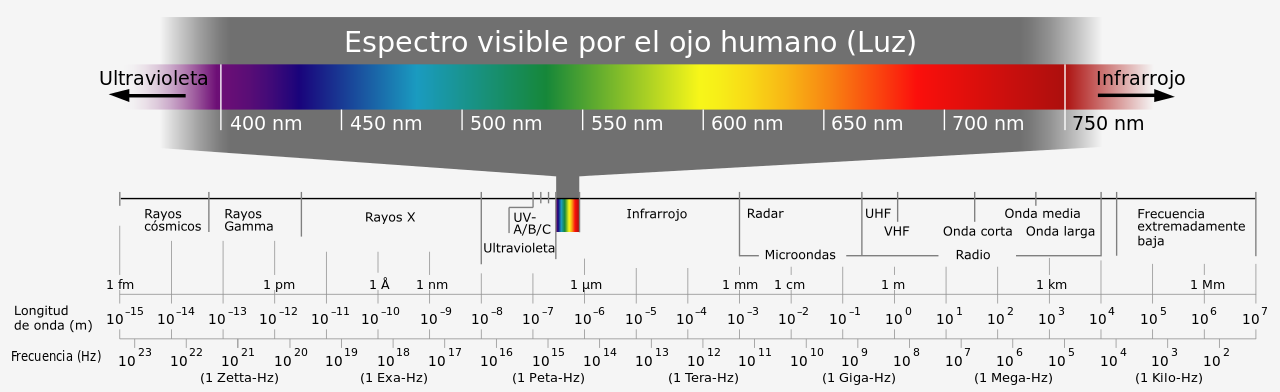
\includegraphics[scale=.3]{images/espectro}
  \caption{\em Luz visible por el ojo humano en el espectro electromagnético~\citep{Horst2006}. }  
  \label{fig:espectro}
\end{figure}

Cuando la luz incide sobre un objeto, puede ser absorbida y la energía, convertida en calor, puede atravesarlo o bien ser reflejada por el mismo. El color de un objeto depende de la cantidad relativa de luz absorbida y de luz reflejada, los objetos de colores reflejan luz que tiene una mayor densidad ondas para ciertas de longitudes de onda del espectro visible que en otras. 

\begin{figure}[htc]
  \centering
  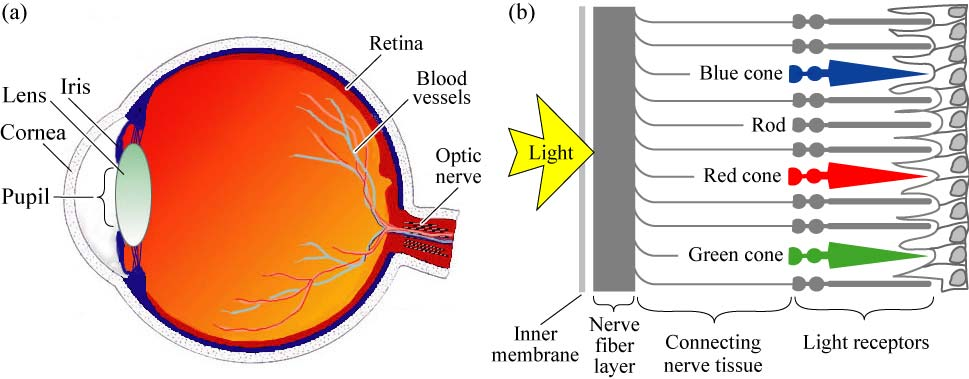
\includegraphics[scale=.4]{images/ojo}
  \caption{\em A la izquierda anatomía del ojo humano, a la derecha esquema de la retina, que muestra conos y bastones. Adaptado de \cite{Britannica1994}}  
  \label{fig:ojo}
\end{figure}

La luz debe atravesar el ojo (figura~\ref{fig:ojo}), desde la córnea hasta la retina, generando un enfoque con la menor distorsión posible. La retina consta de diez capas que trabajan en conjunto con la finalidad de generar el impulso nervioso que se dirigirá a la corteza cerebral para reconocer finalmente una imagen. El ojo es capaz de absorber la luz en su totalidad e impedir la reflexión en su interior, siendo ésta transmitida hacia la segunda capa de la retina, conformada por los foto-receptores, células sensoriales sensibles a la intensidad y longitud de onda de la luz. Existen dos tipos; conos y bastones. Los bastones, elementos encargados de la visión con poca luz, son acromáticos, es decir, sólo permiten captar la luz en tonalidades de gris. Tienen un pico de sensibilidad aproximado en los 500 nm, como se puede observar en la figura~\ref{fig:cono} (curva R). Los conos por su parte, son los elementos encargados de activarse en condiciones de alta intensidad lumínica, por lo que generan la visión cromática diurna. Hay tres clases de conos, distintos entre sí por el tipo de pigmento fotosensible que contienen. Los pigmentos en los tres tipos de conos contienen picos de absorción de luz según la longitud de onda. Éstos se encuentran aproximadamente en 420 nm (receptores para el violeta – azul, conos S), 530 nm (receptores para el azul – verde, conos M) y 560 nm (receptores para el amarillo – verde, conos L). Los tres grupos de conos mezclados generan el espectro completo de luz visible. En capas posteriores se codifica la información recibida, la cual es enviada a través de dos nervios ópticos por cada ojo en dirección hacia el cerebro.

\begin{figure}[htc]
  \centering
  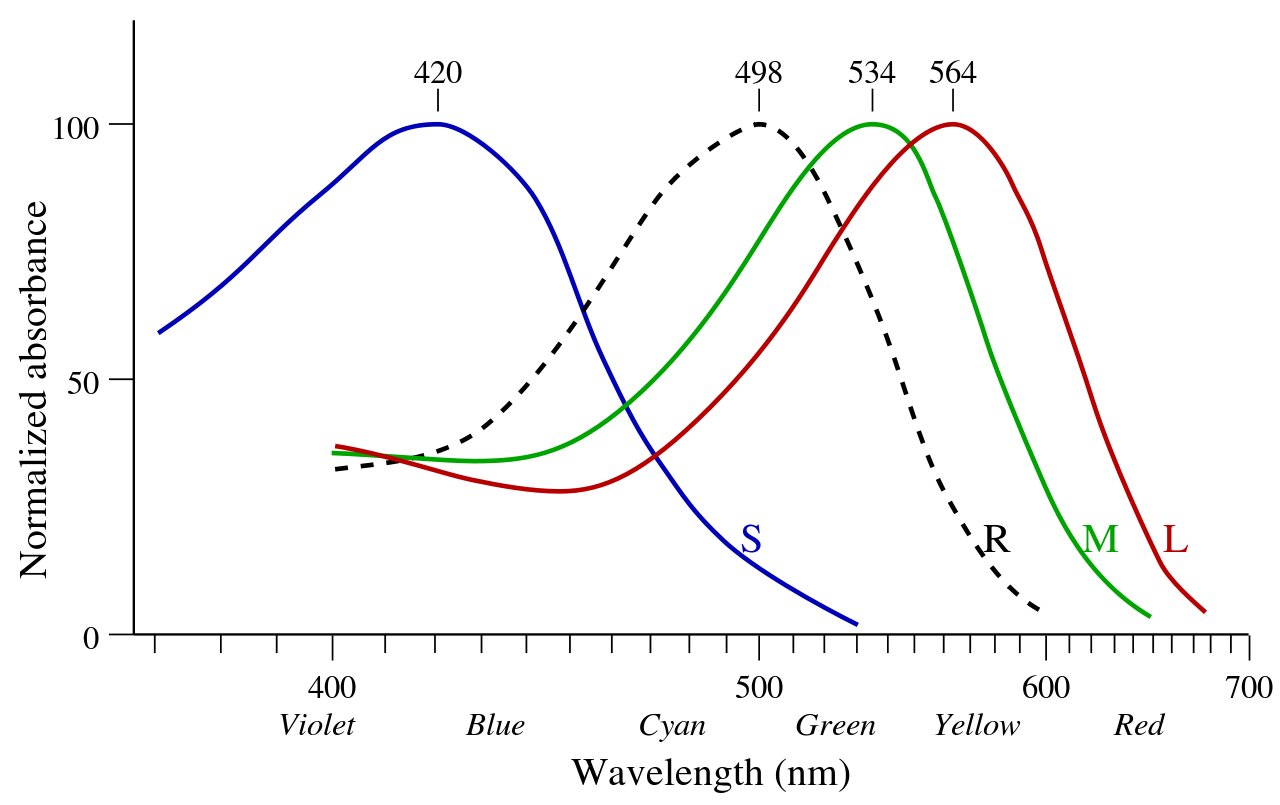
\includegraphics[scale=.3]{images/cono}
  \caption{\em Curvas de absorción espectral de corta (S), mediana (M) y larga (L) longitud de onda, según pigmentos de células cono y bastones (R) humano. Adaptado de \cite{Bowmaker1980}}  
  \label{fig:cono}
\end{figure}

En su trayectoria, los dos nervios ópticos centrales se entrecruzan, para generar procesamiento de información de ambos ojos en cada hemisferio cerebral, tal como puede observarse en los trayectos en verde en la figura~\ref{fig:cerebro}. Este proceso es importante para la visión de profundidad. Posteriormente se dirige a través del tracto óptico, información proveniente de ambos ojos hacia la corteza visual primaria, ubicada en el lóbulo occipital. Desde allí, se comunican con la corteza visual de asociación, responsables del reconocimiento de objetos y de la percepción del color.

\begin{figure}[htc]
  \centering
  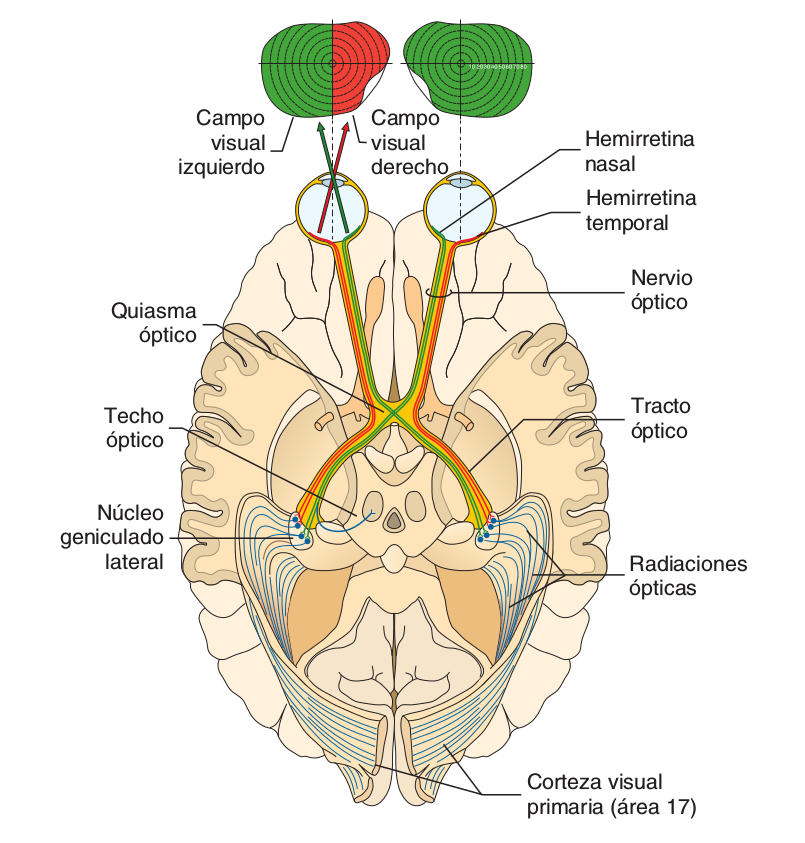
\includegraphics[scale=.3]{images/cerebro}
  \caption{\em Principales vías visuales. Obtenido de \cite{Battaglini2010}}  
  \label{fig:cerebro}
\end{figure}

Este proceso toma en un ser humano desde fracciones hasta unos cuantos segundos, sin embargo, utilizar un computador para realizar dicho ejercicio se torna una tarea desafiante. La visión por computador es un área de estudio que trata este problema. Corresponde a un campo dentro de la inteligencia artificial enfocado al modelamiento matemático de los procesos de percepción visual de los humanos. En general está enfocada al procesamiento de las imágenes con el fin de obtener información simbólica de estas. Algunas de las tareas que pretende resolver la visión por computador son determinar la posición, la distancia o contar los objetos en una imagen. En palabras sencillas la visión por computador se enfoca en la tarea de ``enseñar a ver a los computadores''.

\begin{figure}[htc]
  \centering
  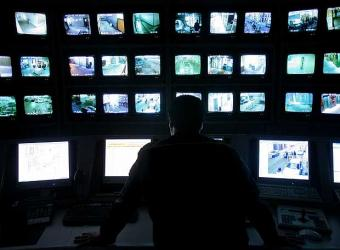
\includegraphics[scale=.42]{images/vigilancia}
  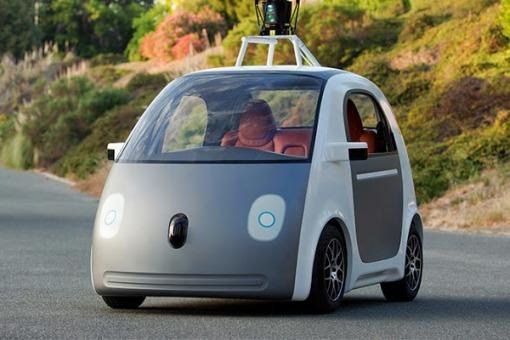
\includegraphics[scale=.36]{images/googleauto}
  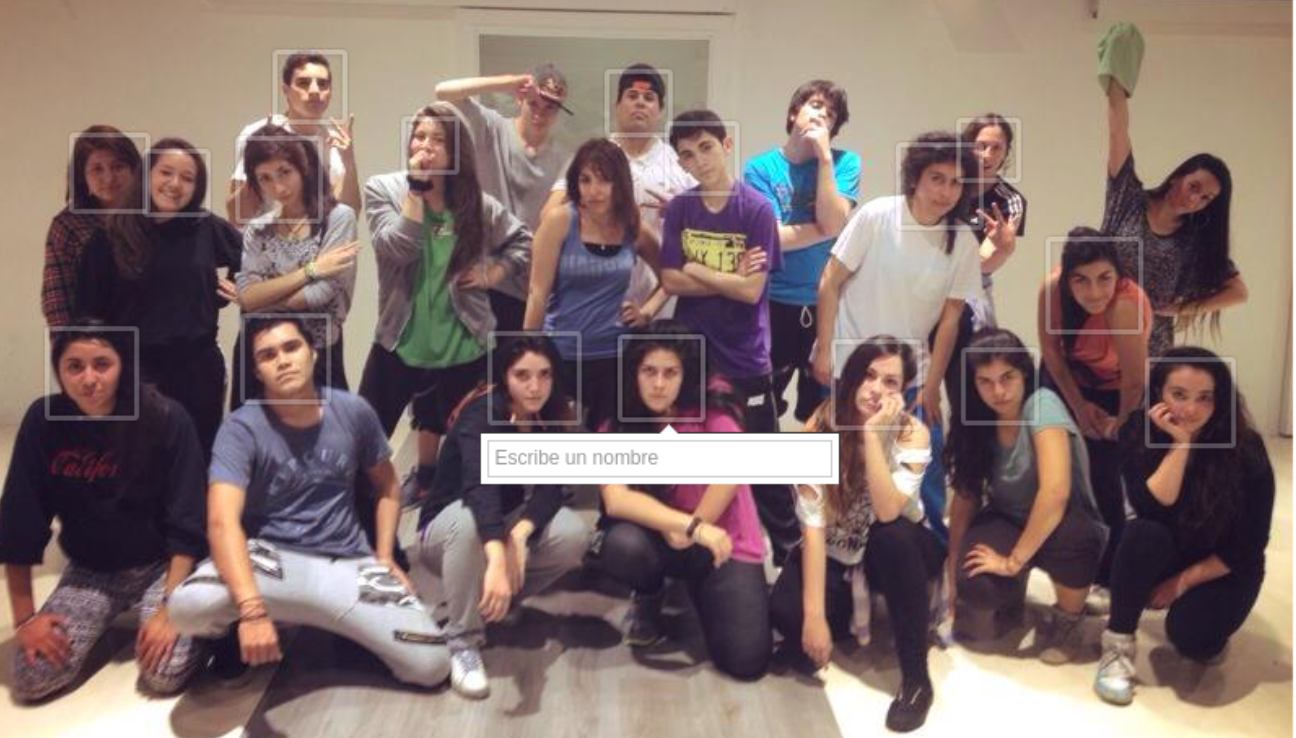
\includegraphics[scale=.25]{images/faces}
  \caption{\em Algunos ejemplos de aplicaciones de la visión por computador. Arriba a la izquierda sistema de video vigilancia. Arriba a la derecha auto autónomo inteligente de Google. Abajo reconocedor de rostros de Facebook}  
  \label{fig:ejemplosaplicacion}
\end{figure}

Existe una gran variedad de investigaciones en el área de la visión por computador, pero sin duda uno de las principales tareas corresponde a la detección de diferentes tipos de objetos en imágenes y videos. El desarrollo de esta capacidad en un computador abre las puertas a un gran número de aplicaciones en variadas áreas como; interacción humano-computador, robótica, análisis automático de contenido en medio digitales, automatización de proceso de manufactura y automóviles autónomos inteligentes.

El presente trabajo centra su foco en un problema particular dentro de la detección de objetos, el cual es, la detección de personas. Y más aún un subproblema dentro de la detección de personas, la caracterización de la ``Sensibilidad Espacial''. Para solucionar el problema de la detección de personas se ha propuesto diversidad de enfoques. Algunos de los enfoques más relevantes del problema son la detección holística \citep{dalal2006}  que corresponde a la consideración de la persona de cuerpo completo como un todo, la detección basada en partes \citep{nevatia2005} detectando partes de un objeto por separado y luego reuniéndolas, o una mezcla de estos enfoques \citep{leibe2005,yu2011}.

El problema de determinar la existencia de un peatón en una determinada ventana de clasificación se encuentra bien estudiado. Sin embargo, al considerar un enfoque de detección basado en un ventana deslizante que se desplaza por la imagen realizando clasificaciones para encontrar a un peatón, surge la posibilidad de que se realicen múltiples detecciones. Esta probabilidad aumenta cuanto más cerca este la ventana respecto del objeto a detectar. Como es preciso evitar que esto ocurra es necesario estudiar el comportamiento de la salida del clasificador, especialmente en la cercanía del peatón. A las variaciones en la salida mientras se desplaza la ventana de clasificación se le denomina ``Sensibilidad Espacial''.

Como se explica con detalle más adelante, la Sensibilidad Espacial es un concepto clave dentro del desarrollo de este trabajo ya que es importante su caracterización (para una determinada combinación de descriptor y máquina de aprendizaje) de modo que sea posible determinar cual es el grado de sintonización del clasificador respecto de los objetos que se encuentra clasificando.

\section{Descripci\'on del problema}
\label{intro:problema}

Determinar la existencia de un peatón en una sección de una imagen es un problema bastante estudiado. Sin embargo, dentro de la detección de peatones (donde están los peatones en una imagen) se encuentra el subproblema del comportamiento del clasificador en el momento de encontrarse evaluando la vecindad cercana al peatón. A este problema lo denominamos caracterización de la sensibilidad espacial.

Un clasificador de personas (o cualquier otro tipo de objeto para los cuales haya sido entrenado) evalúa la presencia de un peatón en la imagen analizando la información tomada de una ventana o cuadro que se desliza por dicha imagen y entrega como resultado la determinación de la existencia de un peatón o no además de un valor para el nivel de confianza con el cual el clasificador asegura que se trata de un peatón.

\begin{figure}[htc]
  \centering
  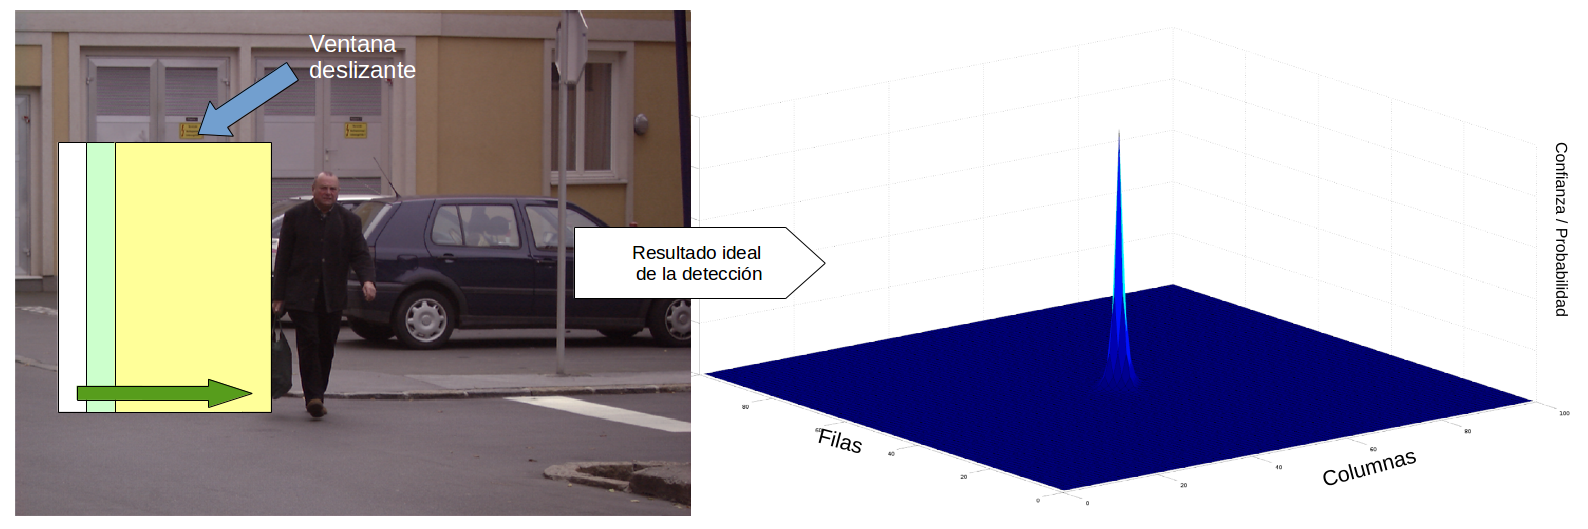
\includegraphics[scale=.3]{images/ejloesp}
  \caption{\em Escenario ideal en la salida de un clasificador. A la izquierda detección con la ventana deslizante. A la derecha salida ideal.} 
  \label{fig:ejloesp}
\end{figure}


En forma ideal, la confianza de la respuesta del clasificador sólo debe ser muy alta cuando la ventana evaluada se encuentra frente a frente al peatón y no cuando se encuentra en su cercanía. En este último caso, la confianza de su respuesta debe ser muy baja. En la figura~\ref{fig:ejloesp}, a la izquierda se observa en color verde el desplazamiento de la ventana de clasificación acercándose al momento en que la ventana se encuentre completamente frente al peatón, a la derecha se muestra el resultado obtenido posterior a la clasificación desplazando la ventana por toda la vecindad. Si se tratase de un buen clasificador; en un escenario ideal el resultado obtenido debería asemejar a la función impulso. Esta es entonces una posible representación de un escenario ideal.


\section{Soluci\'on propuesta}
\label{intro:solucion}
% ***SAV here 

\subsection{Características de la solución propuesta}

Para caracterizar la sensibilidad espacial se propone por una parte una métrica y por otra una metodología de evaluación. Tanto la métrica como la metodología de evaluación se construirá de modo que pueda ser implementada basada en la biblioteca de visión por computador OpenCV. Esta biblioteca contiene implementaciones de varios algoritmos de visión por computador además de herramientas para el manejo de imágenes en general. También existen desventajas en la utilización de OpenCV ya que la documentación asociada a la biblioteca se encuentra incompleta y presenta una cantidad apreciable de errores, lo que dificulta su utilización.

La evaluación será desarrollada en torno a una métrica propuesta, lo que se construirá en una serie de siete pasos con la culminación del cálculo de la propia métrica. Es importante que durante la evaluación sea posible obtener resultados parciales para comprobar el avance y contrastar diferencias. El enfoque principal de la evaluación será realizar una detección del peatón en base al modelo de la ventana deslizante en su vecindad. 

Por el lado de la métrica es importante que cumpla con la mayor cantidad de características deseables de una métrica. Algunas de estas características son.

% ***SAV. A lo mejor debes tener un poco de cuidado con la palabra "metrica" ya que matematicamente es bastante más precisa de lo que usas (ver http://es.wikipedia.org/wiki/Espacio_m%C3%A9trico) . A lo mejor debes aclarar que lo que buscas es una "medida" más que una metrica estricta o mejor aun si demuestras que tu metrica es de verdad una metrica (no debiera ser muy complicado) ***DQ Revisado

\begin{itemize}
\item Fácil de medir: toda métrica debes aspirar a ser fácil de medir, cuanto más fácil más extendido será su uso y más rápido será perfeccionada.
\item Linealidad: idealmente la métrica debe ser lineal respecto de la característica a medir.
\item Fiabilidad: la métrica debe aumentar o disminuir su valor conforme aumenta o disminuye la propiedad medida respectivamente. También esta variación puede ser inversa \ie mientras una aumenta la otra disminuye.
\item Repetibilidad: al realizar el mismo experimento en varias ocasiones el resultado es el mismo \ie la métrica tiene un resultado determinista.
\item Consistencia: al cambiar el sistema y la configuración la métrica debe mantener su significado y su unidad de medida.
\item Independencia: la métrica no debe estar influenciada para obtener resultados de algún tipo en específico.
\end{itemize}

Además, matemáticamente una métrica es una función distancia asociada a un espacio métrico que debe cumplir cuatro axiomas, estos son: positividad, identidad de los indiscernibles, simetría, desigualdad triangular. Entonces es necesario demostrar que la métrica diseñada cumpla con estos axiomas. 

\subsection{Propósitos de la solución}

El propósito de la solución es contribuir a la investigación en detección de peatones. Para esto se caracterizan nuevos aspectos del problema antes no tratados. La detección de peatones es un problema muy amplio por lo que una contribución tiene repercusión a nivel de una gran gama de aplicaciones distintas. 
De forma directa esta investigación realiza un aporte dentro del proyecto Fondecyt Regular OBSERVE (N'o 1140209), orientado al reconocimiento de acciones humanas dentro del transporte público.

Otro propósito lateral es aportar en problemas similares de detección no necesariamente relacionada con personas \ie detección de objetos en general. Muchos algoritmos de detección de objetos están basados en la misma estructura que un detector de personas por lo que es perfectamente aplicable esta solución en esos problemas.

\section{Objetivos y alcance del proyecto}
\label{intro:objetivos}

\subsection{Objetivo general}

Desarrollar y probar una métrica que permita la comparación de la sensibilidad espacial entre diferentes esquemas descriptor-clasificador, encontrando aquel que reduce detecciones múltiples en la vecindad del peatón utilizando el set de datos de referencia INRIA.

\subsection{Objetivos específicos}

Para la consecución del objetivo general, se plantean las siguientes metas intermedias:

\begin{enumerate}

\item Proponer un modelo matemático que permita generar un métrica que describa la sensibilidad espacial.
\item Evaluar la sensibilidad espacial de un clasificador en la vecindad de un peatón.
\item Desarrollar un software modular que permita automatizar la evaluación de la sensibilidad espacial para cada peatón en un conjunto de \textit{``ground truths''}. 
\item Determinar cuál de los clasificadores posee la mejor sensibilidad espacial para minimizar detecciones múltiples de peatones en el set de datos INRIA.

\end{enumerate}

\subsection{Alcances y limitaciones}

Los alcances y limitaciones listados a continuación ayudan a determinar la frontera del proyecto. 

\subsubsection{Alcances}

Para efectos de la evaluación de los clasificadores humanos se utilizó un set de datos único, que corresponde al set de datos INRIA. Este estudio comprende la caracterización de la sensibilidad desde un enfoque métrico \ie el objetivo es medir la sensibilidad espacial. Esta incluido en el desarrollo una etapa de para la proposición de la métrica, una para la evaluación diseño del proceso de evaluación, una etapa para el desarrollo de software y finalmente una etapa para realizar el análisis comparativo y la escritura del presente documento.

\subsubsection{Limitaciones}

\begin{itemize}

\item Está fuera de los alcances del proyecto el desarrollo de nuevas técnicas o algoritmos de clasificación, se busca probar los algoritmos existentes en su estado original o modificar sus variables de manera que mejore su sensibilidad espacial según el indicador obtenido.

\item La solución de software corresponde a un programa para línea de comandos desarrollado para sistema operativo Linux y no se considera dentro de la solución el desarrollo de ningún tipo de interfaz gráfica adicional.

\item Se realizó el análisis de 8 combinaciones de descriptor-clasificador en diferentes escalas dentro de las cuales algunas se encuentran implementadas y otras deberán ser implementadas previo a realizar las pruebas.

\item Finalmente la solución se validó ya que el software construido tiene la capacidad de probar diferentes clasificadores humanos entregando sus resultados, el valor del indicador comparativo y es posible determinar la sensibilidad espacial de cada uno permitiendo su comparación.

\end{itemize}

%**DQ REVISAR METODOLOGÍA!!

\section{Metodolog\'ia y herramientas utilizadas}
\label{intro:metodologia}

El desarrollo del trabajo se realiza fundamentalmente como un proceso de investigación, el cual lleva incorporado dentro de si una etapa de desarrollo de software. Por esta razón es importante conocer el marco metodológico asociado a la investigación y en forma secundaria aquel relacionado con el desarrollo de software.
El proceso de investigación gira en torno a la posibilidad de evaluar la sensibilidad espacial dada una clasificación en la vecindad de un peatón y comparar este resultado con el resultado obtenido por un clasificador diferente.

\subsection{Metodología para la investigación}

La metodología de investigación funciona como marco general para el desarrollo por lo que es necesario cumplir un objetivo científico \ie describir y evaluar la sensibilidad espacial a través de una métrica propuesta. Para esto se utilizará el método científico.

Las actividades dentro de esta metodología son las que se describen a continuación.

\begin{itemize}
\item Formulación de la hipótesis. 
La hipótesis formulada tiene relación directa con el correcto funcionamiento de la métrica la que debe permitir diferenciar resultados de un conjunto descriptor-clasificador de los de otro. Para esto es necesario plantear una hipótesis como la siguiente.
\subitem ``La métrica propuesta permite la comparación de los resultados de sensibilidad espacial entregando resultados con diferencias estadísticamente significativas''
\item Marco teórico. Explicar conceptos básicos sobre visión por computador y cuales son las principales áreas de estudio relacionadas. Exponer la investigación sobre detección de peatones así como las herramientas, métodos y enfoques asociados.
\item Diseño de la solución. Realizar la proposición de una métrica que permita evaluar la sensibilidad espacial y diseñar el proceso de evaluación con el cual se validará. Además se describirán las herramientas seleccionadas para la evaluación de la métrica y se fundamentará las razones de su elección.
\item Análisis y presentación de los resultados. Se realizará el análisis de los resultados obtenido mostrando el proceso de comparación a nivel gráfico y por otra parte el análisis estadístico el cual permite finalmente la aceptación o rechazo de la hipótesis planteda.   
\item Conclusiones. Se presentan las conclusiones sobre los resultados obtenidos.

\end{itemize}

\subsection{Metodolog\'ia para el desarrollo de software}

%%POR COMPLEMENTAR !!!!!

Dada la necesidad de construir una solución de software que permita incorporar tanto en el proceso de detección de peatones como en la evaluación de la sensibilidad espacial. Sin embargo, esta metodología debe adaptarse a las necesidades cambiantes de la investigación y tener por objetivo principal obtener rápidamente los resultados necesarios para probar adecuadamente la hipótesis planteada.

En primer lugar, dada la naturaleza de este trabajo, el equipo de desarrollo se compuso de un solo integrante – el autor – quien además funcionó como cliente conjunto con la colaboración del profesor guía. Entonces es el autor quien identifica los requerimientos asociados a la solución de software a desarrollar y quien debe darle posterior cumplimiento. En segundo lugar se considera que las necesidades de documentación del software eran necesarias en lo que respecta a usuarios y desarrolladores externos que desearan observar su trabajo, pero que el número de artefactos a utilizar no debía ser extenso, principalmente por la poca practicidad que representa el uso de muchos de ellos. Se prefirió entonces la utilización de una metodología ágil que permitiera optimizar la utilización del recurso tiempo y que fuera adaptable a cada que pudiera presentarse situación. Es por esta razón que se escogió como metodología de desarrollo a \textit{Extreme Programming} (XP) adaptado a una sola persona.

Se justifica la elección de XP debido principalmente al hecho de que constituye una metodología ágil que permite centrar el foco principalmente en el desarrollo de la solución más que en la construcción de artefactos, se puede adaptar de manera sencilla a un equipo unipersonal donde se cumple con la particularidad además de que el cliente y el equipo de desarrollo son la misma persona, asegurando de esta forma un 100\% de disponibilidad y comunicación entre ambos roles de la metodología (que asume que el cliente está siempre presente durante el desarrollo del proyecto).

Si bien el proyecto no se consideró como de alto riesgo, la metodología, gracias a los ciclos de desarrollo cortos y pruebas constantes, permite minimizar el riesgo asociado al desarrollo detectando y controlando los fallos en el desarrollo, tanto a nivel de código como de planificación de manera temprana y con consecuencias reducidas, presentando una considerable ventaja por sobre otras metodologías bajo las circunstancias en las cuales se llevó a cabo el desarrollo.

\subsection{Herramientas de desarrollo}

Para el desarrollo de este proyecto de título fue necesaria la utilización de herramientas que permitieron llevar a cabo tanto la construcción del software relacionado como la redacción del presente documento.
En particular para el desarrollo del software se utilizaron las siguientes herramientas.

\begin{itemize}
  \item SublimeText 3 - Procesador de texto con variadas utilidades para la producción de código.
  \item C++ 11 - Lenguaje de programación C++ en su estándar del año 2011 ISO/IEC 14882:2011.
  \item OpenCv 2.4 - Biblioteca \textit{open source} para el desarrollo de aplicaciones de visión por computador, con soporte para C, C++ y Python.
  \item Boost C++ Libraries 1.5 - Biblioteca para C++ con importantes mejoras para el lenguaje.
  \item Python - Lenguaje de programación Python en su versión 2.7.6.
  \item Octave - Lenguaje de programación interpretado de alto nivel, similar a MATLAB, en su versión 3.8.1.
  \item Linux Mint 17 - Sistema operativo Linux basado en Ubuntu 14.04.
  \item Git - Herramienta para el control de versión de código, se utilizó el servicio prestado por Github para mantener una copia en línea.
  \item OpenMP - API para programación paralela para lenguaje de programación C/C++.
  \item SPSS 22.0 - Software para análisis estadístico predictivo de IBM 
  \item STATISTICA 10.0 - Software para análisis estadístico predictivo de StatSoft - Dell Software
\end{itemize}

Para la escritura del presente documento se utilizaron las siguientes herramientas

\begin{itemize}
\item Latex - Para el procesamiento, compilación del texto y transformación en pdf.
\item Dropbox - Para almacenamiento en línea y control de versión.
\item Sharelatex - El servicio de sharelatex provee un entorno de escritura además de las facilidades para la compilación y sincronización con dropbox.
\end{itemize}


\section{Organizaci\'on del documento}
\label{intro:organizacion}

%*** agregar mención capitulo experimento

El presente trabajo está dividido en siete capítulos considerando éste como el primero. En el capítulo~\ref{cap:preliminares} se presentará el marco teórico y el estado del arte en torno al problema antes descrito. Luego de definido el marco teórico es importante definir los lineamientos sobre el proceso experimental de esta investigación, lo que se describirá en el capítulo~\ref{cap:experimento}. A continuación en el capítulo~\ref{cap:metricas} se analizará el proceso por el cual fueron seleccionadas las métricas de sensibilidad espacial y como se construye cada una de estas. A continuación en el capítulo~\ref{cap:caract} se evaluarán las técnicas utilizadas para la extracción de características de las imágenes en particular del algoritmo HOG. En el capítulo \ref{cap:eval} se expone el proceso de evaluación realizado a través del  cual se obtuvieron los resultados que son expuestos en el capítulo \ref{cap:analisis}. Además en el capítulo \ref{cap:analisis} se realiza el análisis comparativo de los clasificadores analizados. Finalmente en el capítulo \ref{cap:conclusiones} se realiza una breve discusión, se concluye sobre los resultados obtenidos y la proyección de estos para futuras investigaciones.

Para mejorar la lectura del presente documento se puede encontrar cuatro anexos los cuales contienen, un glosario con explicaciones de los conceptos mas importantes, el manual de usuario del software desarrollado, los gráficos obtenidos al realizar análisis de métricas y finalmente los gráficos obtenidos para el análisis comparativo. 
